\documentclass[tikz,border=10pt]{standalone}

\usepackage{xcolor}
\usetikzlibrary{positioning, arrows.meta, shapes.geometric}

% Define el color si no lo tienes en este fichero standalone
\definecolor{blueColor}{RGB}{0,70,140}

\begin{document}

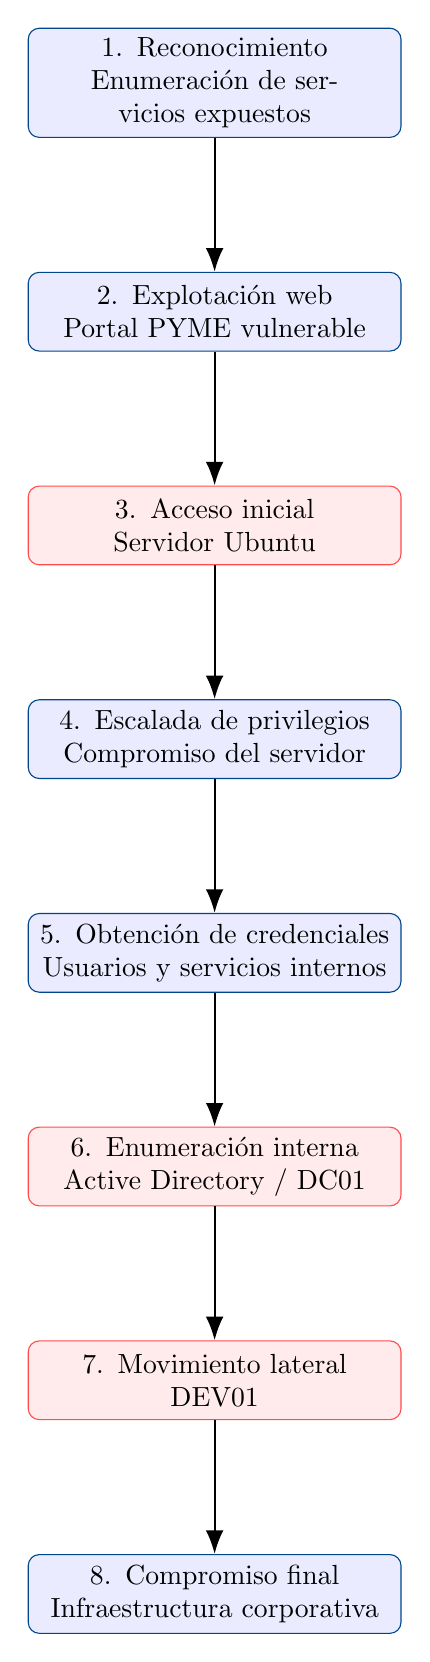
\begin{tikzpicture}[
    node distance=1.7cm,
    fase/.style={
        rectangle,
        rounded corners,
        draw=blueColor,
        fill=blue!8,
        text width=4.5cm,
        align=center,
        minimum height=1cm
    },
    sistema/.style={
        rectangle,
        rounded corners,
        draw=red!70,
        fill=red!8,
        text width=4.5cm,
        align=center,
        minimum height=1cm
    },
    flecha/.style={
        -{Latex[length=3mm]},
        thick
    }
]

    \node[fase] (recon) {1. Reconocimiento\\Enumeración de servicios expuestos};
    \node[fase, below=of recon] (web) {2. Explotación web\\Portal PYME vulnerable};
    \node[sistema, below=of web] (ubuntu) {3. Acceso inicial\\Servidor Ubuntu};
    \node[fase, below=of ubuntu] (priv) {4. Escalada de privilegios\\Compromiso del servidor};
    \node[fase, below=of priv] (creds) {5. Obtención de credenciales\\Usuarios y servicios internos};
    \node[sistema, below=of creds] (ad) {6. Enumeración interna\\Active Directory / DC01};
    \node[sistema, below=of ad] (lateral) {7. Movimiento lateral\\DEV01};
    \node[fase, below=of lateral] (dominio) {8. Compromiso final\\Infraestructura corporativa};

    \draw[flecha] (recon) -- (web);
    \draw[flecha] (web) -- (ubuntu);
    \draw[flecha] (ubuntu) -- (priv);
    \draw[flecha] (priv) -- (creds);
    \draw[flecha] (creds) -- (ad);
    \draw[flecha] (ad) -- (lateral);
    \draw[flecha] (lateral) -- (dominio);

\end{tikzpicture}

\end{document}